% Chapter Template

\chapter{Introduction to Industrial Training} % Main chapter title
\graphicspath{{Pictures/Chapter1}}
\label{Chapter 1} % Change X to a consecutive number; for referencing this chapter elsewhere, use \ref{ChapterX}

\lhead{Chapter 1. \emph{Introduction to Industrial Training}} % Change X to a consecutive number; this is for the header on each page - perhaps a shortened title

%----------------------------------------------------------------------------------------
%	SECTION 1
%---------------------------------------------------------------------------------------
\section{CIT}
The Central Institute of Technology Kokrajhar (CITK) is a public technical university established in 2006 and owned by the Government of India. It is located in Kokrajhar, Assam, India. The institute is spread across 300 acres (1.2 km2) in Kokrajhar and offers Bachelor of Technology (B.Tech.), Bachelor of Design (B.Des.), Master of Technology (M.Tech.), Master of Design (M.Des.), PhD, and Diploma programs in various disciplines.\cite{enwiki:citk}
%----------------------------------------------------------------------------------------
%	SECTION 2
%---------------------------------------------------------------------------------------
\section{NIELIT Guwahati}
National Institute of Electronics \& Information Technology (NIELIT), formerly known as the DOEACC Society, is a society that offers Information Technology and Electronics training at different levels.

\begin{figure}[!htbp]
\centering
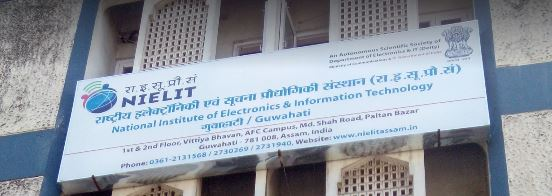
\includegraphics[width=15cm]{nielit.jpeg}
\caption{NIELIT Guwahati}
\label{fignielit}
\end{figure}

It is associated with the Ministry of Electronics and Information Technology of the Government of India.\cite{enwiki:nielit} \par

NIELIT Guwahati is located at 1st \& 2nd floor, Vittiya Bhavan,AFC Building, Md. Shah Road Paltan Bazar, Guwahati - 781008, ASSAM Phone:- 0361-2730269

%----------------------------------------------------------------------------------------
%	SECTION 3
%---------------------------------------------------------------------------------------
\section{About Boot Camp}
Enter the contents here daywise ....
